\documentclass[tikz,border=2pt]{standalone}
\usepackage{amsmath}
\usetikzlibrary{arrows.meta}
\begin{document}
% Pure endowment of 1000 at n = 10 with i = 0.05 and 10p_x = 0.8: the insurer pays 1000 at time 10
% only if T_x > 10 (probability 0.8) and nothing otherwise, so the APV is 1000 v^10 (0.8) ~ 491.13.
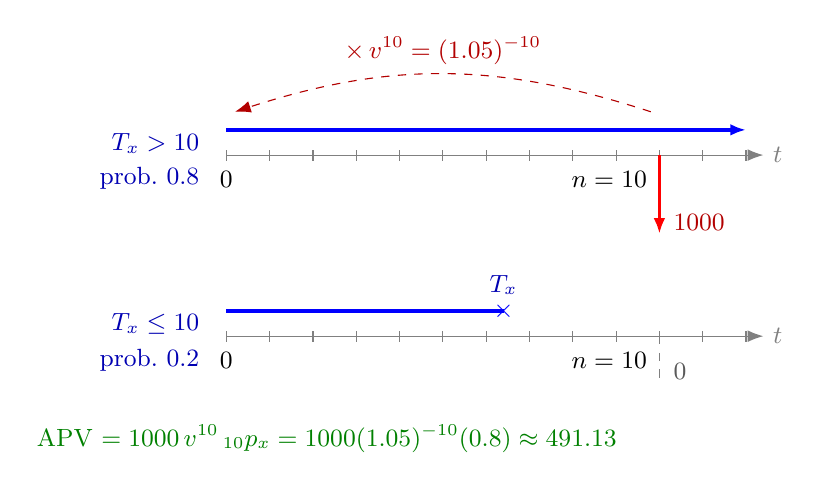
\begin{tikzpicture}[font=\small, >={Latex[length=2mm]}, x=0.55cm]
  % row 1: survives to n
  \draw[gray, ->] (0,0) -- (12.4,0) node[right] {$t$};
  \foreach \t in {0,...,12} \draw[gray] (\t,-0.07) -- (\t,0.07);
  \node[below] at (0,-0.08) {$0$};
  \node[anchor=north east, xshift=-1pt] at (10,-0.08) {$n=10$};
  \draw[blue, very thick, -{Latex[length=2mm]}] (0,0.32) -- (12,0.32);
  \node[blue!70!black, anchor=east] at (-0.4,0.15) {$T_x>10$};
  \node[blue!70!black, anchor=east] at (-0.4,-0.3) {prob.\ $0.8$};
  \draw[red, very thick, ->] (10,0) -- (10,-1.0);
  \node[red!70!black, anchor=west] at (10.1,-0.85) {$1000$};
  \draw[red!70!black, thin, dashed, ->] (9.8,0.55) to[bend right=18] node[above] {$\times\,v^{10}=(1.05)^{-10}$} (0.2,0.55);
  % row 2: dies before n
  \begin{scope}[yshift=-2.3cm]
    \draw[gray, ->] (0,0) -- (12.4,0) node[right] {$t$};
    \foreach \t in {0,...,12} \draw[gray] (\t,-0.07) -- (\t,0.07);
    \node[below] at (0,-0.08) {$0$};
    \node[anchor=north east, xshift=-1pt] at (10,-0.08) {$n=10$};
    \draw[blue, very thick] (0,0.32) -- (6.4,0.32);
    \node[blue] at (6.4,0.32) {$\times$};
    \node[blue!70!black, above] at (6.4,0.4) {$T_x$};
    \node[blue!70!black, anchor=east] at (-0.4,0.15) {$T_x\le10$};
    \node[blue!70!black, anchor=east] at (-0.4,-0.3) {prob.\ $0.2$};
    \draw[gray, dashed] (10,0) -- (10,-0.6);
    \node[gray!70!black, anchor=west] at (10.1,-0.45) {$0$};
  \end{scope}
  \node[green!50!black, anchor=west] at (-4.6,-3.6) {APV $=1000\,v^{10}\,{}_{10}p_x=1000(1.05)^{-10}(0.8)\approx491.13$};
\end{tikzpicture}
\end{document}
